\subsection{Matching Pennies}

\subsubsection{Background}
In this game, two players each receive a coin and will simultaneously pick either to place it head (H) or tails (T) with their choices unknown to the other. After the players have made their choices, the coins are revealed and the payoffs are give based on the outcome. One player's goal is to match the coin faces (H,H or T,T) and the other is to mismatch the faces (H, T). 

In game theory, this is known as a zero-sum game: When one player wins with a payoff of +1 the other player equally loses with a payoff of $-1$. No pure-strategy Nash equilibrium exists: any best response would be countered by the opposing player's best response. A mixed-strategy Nash equilibrium can be found by randomly picking heads or tails with equal probability.  


\subsubsection{Simulation}
One way to illustrate that a game has an equilibrium strategy is to simulate the game with the players having strategy adjustment functions. It is similar to evolution: the losing player must change his strategy in order to survive. The simulation used for this example has the players start at a given mixed strategy. The players will play twenty games and then check to see if either player lost beyond a preset cutoff (four more than the other or twenty percent). If a player lost too much, then the adjustment function will change the weights of their mixed strategy to favor them and if not the players will continue with their strategies.

The adjustment function in this case is a step function. If a player loses too much then the probabilities of them picking heads or tails is modified by plus or minus five percent to favor their goal (match or mismatch).  Thus over a number of games the adjustment function will add or subtract from the weights till the players continue to play without reaching the cutoff value.  

From Figure 1, the players seem to converge near the mixed strategy of equal weight to heads and tails. The graph shows the players starting at pure opposite strategies and converging to the near the fifty percent heads line. Some variance exists due to the randomness of the simulation, which could possibly be further minimized by increasing the number of games played before checking for the cutoff value.

\begin{figure}[h]
\caption{Convergence Over Time: Players' Probability of Picking Heads}
\hspace*{-2.5cm} 
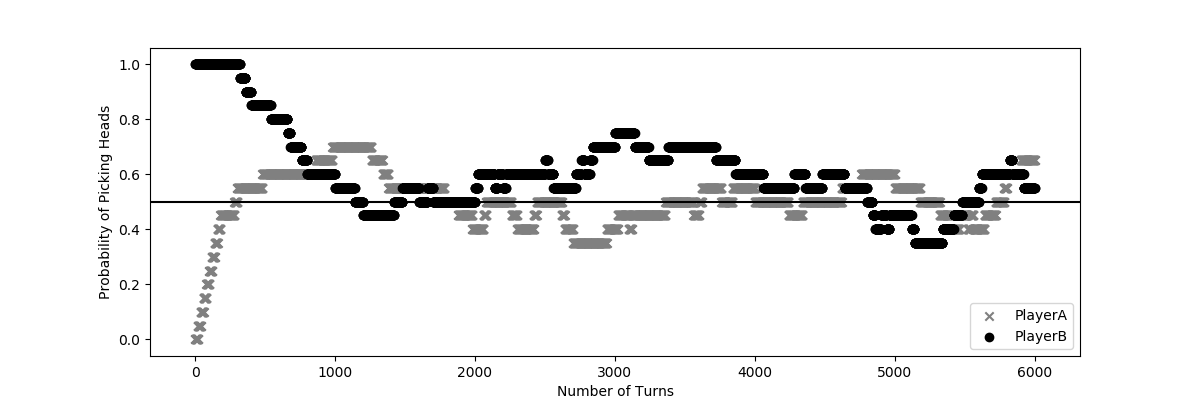
\includegraphics[scale=0.6]{../Figures/scatter_1.png}
\end{figure}

\FloatBarrier
\subsection{Rock-Paper-Scissors}

\subsubsection{Background}
In this game, two players each simultaneously reveal either rock, paper, or scissors. The players then  compare their choices and determine a winner with playoff +1 and a loser with playoff $-1$, a tie gives both players a payoff of 0. Rock beats scissors, scissors beats paper, paper beats rock, and all other combinations are a tie.

As in the matching-pennies game, rock-paper-scissors has no pure-strategy Nash equilibrium, but a mixed-strategy Nash equilibrium can be found by randomly picking rock, paper, or scissors with equal probability.


\subsubsection{Simulation}
A different method to show an equilibrium strategy is to map out all of the possible strategies and create distributions of both of their payoffs. If both players follow the same optimal strategy then the players should have the same payoff distribution. Since both players are the same, disregarding skill, and have access to the same choices and information, they should pick the mixed-strategy Nash equilibrium. 

Any payoff distributions that do not over lap can then be eliminated as possible optimal strategy. If one player is getting a lower payoff on average, then that player would adjust their strategy. This will continue until their payoffs converge. By simulating multiple mixed strategies and creating a distribution of each players payoffs the distributions that overlap should be the equilibrium.

From Figure 2, the players' payoffs converge at the mixed strategy Nash equilibrium weights. The top left graph is an example of when the weights favor player A, the top right favors player B, and the bottom graph is the equilibrium weights. As the weights get closer to equilibrium, the payoff distributions overlap.

\begin{figure}[h]
\caption{Histograms of Player Payoffs for Fixed-Weights}
\hspace*{-1.5cm} 
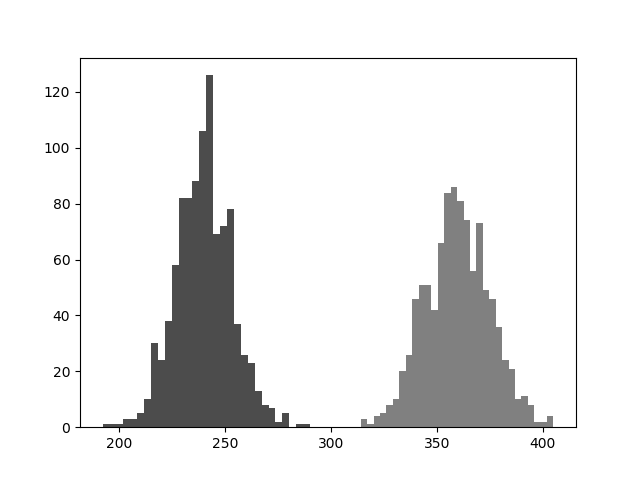
\includegraphics[width=0.6\textwidth]{../Figures/hist_1.png}%
\hfill
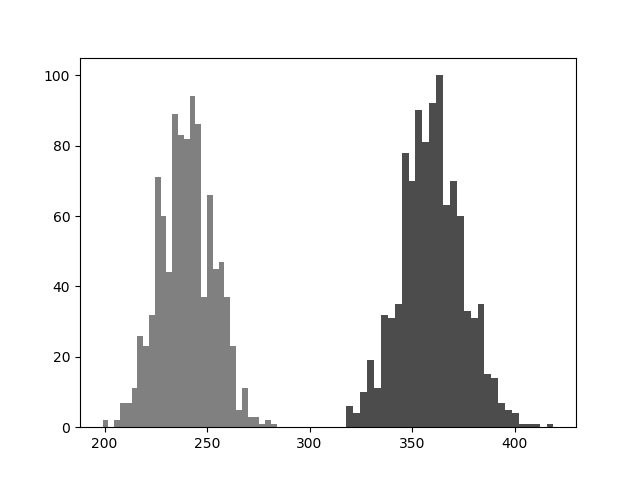
\includegraphics[width=0.6\textwidth]{../Figures/hist_3.png}%
\\
\hspace*{2.5cm} 
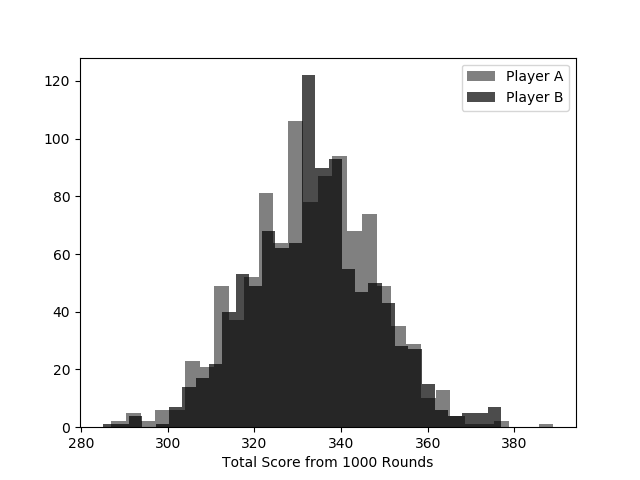
\includegraphics[width=0.6\textwidth]{../Figures/hist_2.png}
\end{figure}





